% ===== DIAGRAM 2: Chain of Responsibility Sequence =====
\documentclass[border=8pt]{standalone}
\usepackage{tikz}
\usetikzlibrary{arrows.meta, positioning, calc}
\usepackage{xcolor}

\definecolor{headingblue}{RGB}{31, 73, 125}
\definecolor{accentblue}{RGB}{70, 130, 180}
\definecolor{classblue}{RGB}{210, 225, 245}

\begin{document}
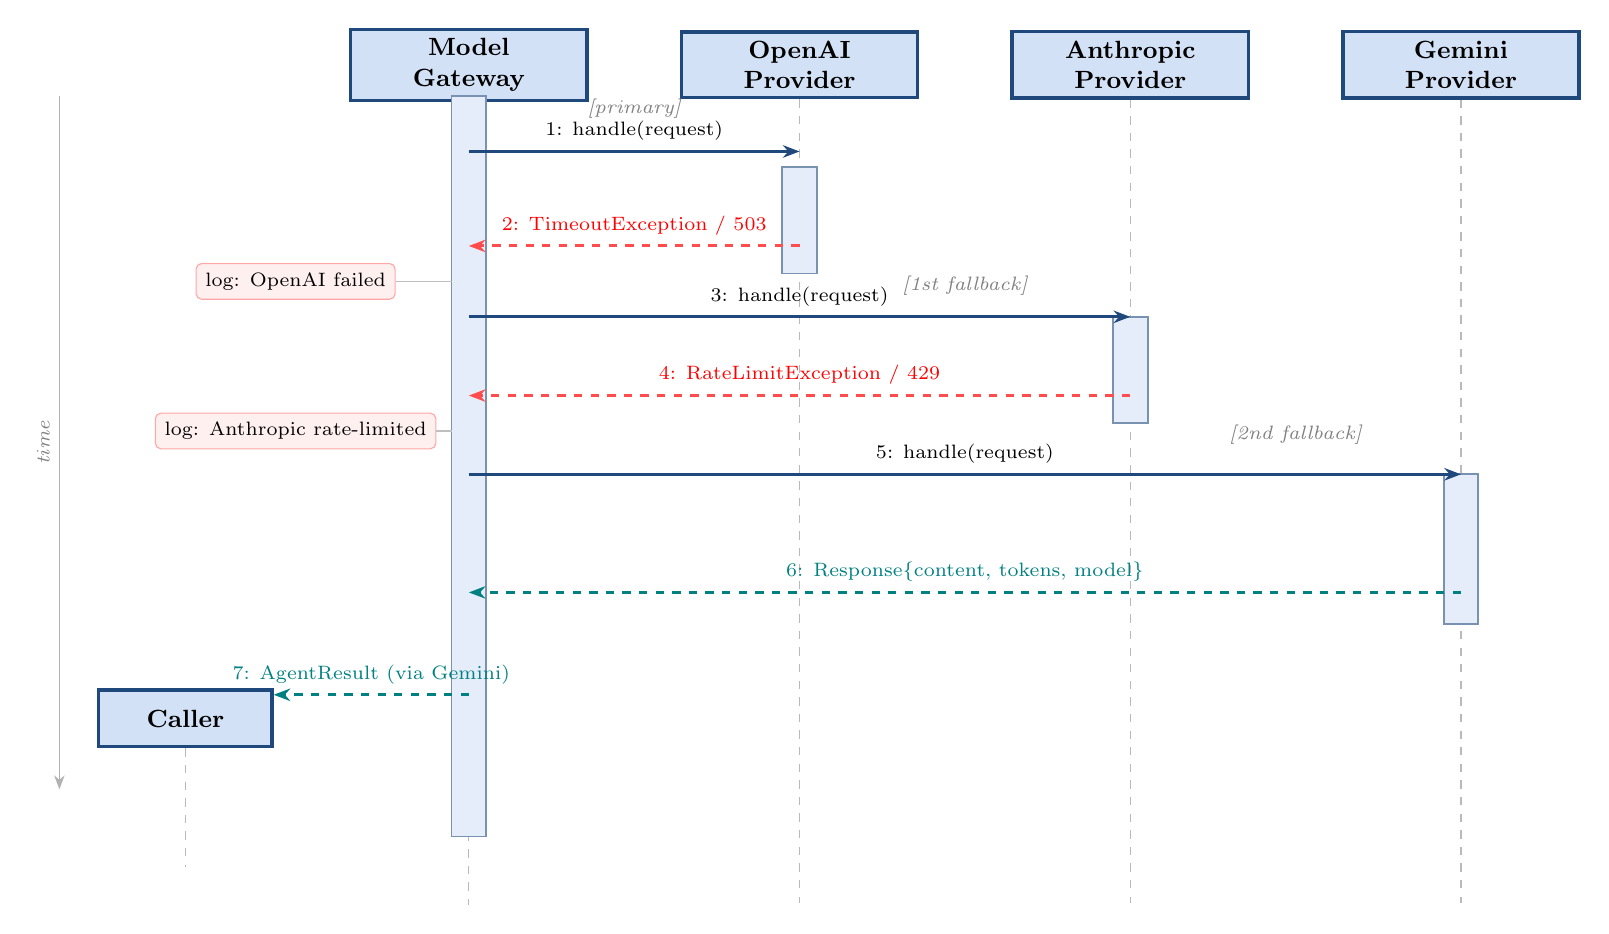
\begin{tikzpicture}[
  actor/.style={
    rectangle, draw=headingblue, line width=1.2pt,
    fill=classblue,
    minimum width=3.0cm, minimum height=0.8cm,
    font=\small\bfseries, align=center
  },
  lifeline/.style={draw=gray!55, dashed, thin},
  msg/.style={-{Stealth[length=6pt]}, line width=1.1pt, draw=headingblue},
  err/.style={-{Stealth[length=6pt]}, line width=1.1pt, draw=red!70, dashed},
  ok/.style={-{Stealth[length=6pt]}, line width=1.1pt, draw=teal, dashed},
  actbox/.style={rectangle, draw=headingblue!60, fill=classblue!60, line width=0.7pt},
]

%% Lifeline heads
\node[actor] (gw)  at (0,0)    {Model\\Gateway};
\node[actor] (oai) at (4.2,0)  {OpenAI\\Provider};
\node[actor] (ant) at (8.4,0)  {Anthropic\\Provider};
\node[actor] (gem) at (12.6,0) {Gemini\\Provider};

%% Lifelines
\foreach \n in {gw, oai, ant, gem} {
  \draw[lifeline] (\n.south) -- ++(0,-10.2);
}

%% Activation boxes
\draw[actbox] (-0.22,-0.40) rectangle (0.22,-9.8);
\draw[actbox] (3.98,-1.30) rectangle (4.42,-2.65);
\draw[actbox] (8.18,-3.20) rectangle (8.62,-4.55);
\draw[actbox] (12.38,-5.20) rectangle (12.82,-7.10);

%% Guard labels
\node[font=\scriptsize\itshape, gray] at (2.1,-0.55)  {[primary]};
\node[font=\scriptsize\itshape, gray] at (6.3,-2.80)  {[1st fallback]};
\node[font=\scriptsize\itshape, gray] at (10.5,-4.70) {[2nd fallback]};

%% Messages
% 1
\draw[msg] (0,-1.10) -- node[above, font=\scriptsize]{1: handle(request)} (4.2,-1.10);
% 2
\draw[err] (4.2,-2.30) -- node[above, font=\scriptsize]{\textcolor{red}{2: TimeoutException / 503}} (0,-2.30);
% log note
\node[draw=red!35, fill=red!6, rounded corners=2pt, font=\scriptsize, align=left]
  (log1) at (-2.2,-2.75) {log: OpenAI failed};
\draw[gray!50, thin] (-0.22,-2.75) -- (log1.east);

% 3
\draw[msg] (0,-3.20) -- node[above, font=\scriptsize]{3: handle(request)} (8.4,-3.20);
% 4
\draw[err] (8.4,-4.20) -- node[above, font=\scriptsize]{\textcolor{red}{4: RateLimitException / 429}} (0,-4.20);
% log note
\node[draw=red!35, fill=red!6, rounded corners=2pt, font=\scriptsize, align=left]
  (log2) at (-2.2,-4.65) {log: Anthropic rate-limited};
\draw[gray!50, thin] (-0.22,-4.65) -- (log2.east);

% 5
\draw[msg] (0,-5.20) -- node[above, font=\scriptsize]{5: handle(request)} (12.6,-5.20);
% 6
\draw[ok]  (12.6,-6.70) -- node[above, font=\scriptsize]{\textcolor{teal}{6: Response\{content, tokens, model\}}} (0,-6.70);

% 7 — return to caller
\node[actor, minimum width=2.2cm, minimum height=0.72cm] (caller) at (-3.6,-8.30) {Caller};
\draw[lifeline] (caller.south) -- ++(0,-1.5);
\draw[ok] (0,-8.00) -- node[above, font=\scriptsize]{\textcolor{teal}{7: AgentResult (via Gemini)}} (caller.east |- 0,-8.00);

%% Time axis
\draw[-{Stealth[length=5pt]}, gray!60, thin] (-5.2,-0.40) -- (-5.2,-9.20)
  node[midway, rotate=90, above, font=\scriptsize\itshape, gray]{time};

\end{tikzpicture}
\end{document}
